 %%%%%%%% ICML 2019 EXAMPLE LATEX SUBMISSION FILE %%%%%%%%%%%%%%%%%
\documentclass{article}
% Recommended, but optional, packages for figures and better typesetting:
\usepackage{microtype}
\usepackage{graphicx}
%\usepackage{subfigure}
\usepackage{booktabs} % for professional tables
% hyperref makes hyperlinks in the resulting PDF.
% If your build breaks (sometimes temporarily if a hyperlink spans a page)
% please comment out the following usepackage line and replace
% \usepackage{icml2019} with \usepackage[nohyperref]{icml2019} above.
\usepackage{hyperref}
% Attempt to make hyperref and algorithmic work together better:
%\newcommand{\theHalgorithm}{\arabic{algorithm}}
% If accepted, instead use the following line for the camera-ready submission:
\usepackage[accepted]{icml2019}

%%% BEGIN our stuff
\RequirePackage[table]{xcolor}
\usepackage{multirow}
\usepackage{makecell}
\usepackage{pifont}% http://ctan.org/pkg/pifont
\newcommand{\cmark}{\ding{51}}%
\newcommand{\xmark}{\ding{55}}%
\usepackage{amsmath,amssymb}
\usepackage{dsfont}
% \usepackage{bbm}
\usepackage{caption,subcaption}
\usepackage[noend]{algpseudocode}  % Note: Had to disable algorithmic in icml2019.sty
\usepackage[12pt]{moresize}

\newcommand{\fix}{\marginpar{FIX}}
\newcommand{\new}{\marginpar{NEW}}
%%% END our stuff

% The \icmltitle you define below is probably too long as a header.
% Therefore, a short form for the running title is supplied here:
\icmltitlerunning{Adaptive Neural Trees}

\begin{document}

 \twocolumn[
 \icmltitle{\Large Supplementary materials: Adaptive Neural Trees\\}
 ]
 \appendix
 

% ------------------------ DO NOT DELETE --------------------------------
% %%% Table that shows the number of parameters for the ablation study %%%%%
% \section{Ablation study of different constituent modules}
% In this section, we investigate the roles of router and transformer modules on the performance of ANTs. 

% \begin{table}[h]
% 	\caption{Ablation study to compare the effects of different components of ANTs on the number of parameters\label{tab:ablationstudy_2}}
% 	\vspace{-2mm}
% 	\scriptsize
%     \center
% 	\begin{tabular}{|l|ccc|ccc|ccc|}
% 		\hline
% 		\multicolumn{1}{|c}{\textbf{Method}} &  \multicolumn{3}{|c|}{\textbf{Params. (Full)}} & \multicolumn{3}{|c|}{\textbf{Params. (Path)}} & \multicolumn{3}{c|}{\textbf{Params. (Path without routers)}}  \\
% 			& Default & No $\mathcal{R}$ & No $\mathcal{T}$ & Default & No $\mathcal{R}$ & No $\mathcal{T}$ & Default & No $\mathcal{R}$  & No $\mathcal{T}$ \\
% 		\hline
% 		ANT-MNIST-A & 101K & 82K & 74K & 85K & 82K & 22K & 49K & 82K & 8K\\
% 	    ANT-MNIST-B & 77K  & 54K & 57K & 51K & 54K & 15K & 44K & 54K & 8K\\
%         ANT-MNIST-C & 40K  & 3K  & 32K & 8K  &  3K &  9K & 6K  & 3K & 8K\\
% 		ANT-CIFAR10-A & 1.4M & 1.0M & 0.8M & 1.0M & 1.0M & 0.5M & 0.8M & 1.0M & 0.03M\\
%         ANT-CIFAR10-B & 0.9M & 0.6M & 0.4M & 0.6M & 0.6M & 0.2M & 0.4M & 0.6M & 0.03M\\
%         ANT-CIFAR10-C & 0.7M & 0.3M & 0.3M & 0.5M & 0.3M & 0.1M & 0.2M & 0.3M & $4\times 10^{-5}$M\\
% 		\hline
% % 		\hline
% % 		ANT-MNIST-A & 101K& 74K  & 82K  & 85K  &  22K    &  82K  & 49K  & 8K & 82K\\
% % 	    ANT-MNIST-B & 77K & 57K & 54K & 51K  & 15K &  54K   & 44K  & 8K & 54K\\
% %         ANT-MNIST-C & 40K & 32K &  3K& 8K   &  9K  &   3K  & 6K   & 8K & 3K\\
% % 		ANT-CIFAR10-A &1.4M & 0.8M   & 1.0M & 1.0M & 0.5M   & 1.0M & 0.8M & 0.03M &1.0M \\
% %         ANT-CIFAR10-B &0.9M & 0.4M  & 0.6M & 0.6M & 0.2M   & 0.6M & 0.4M  & 0.03M  & 0.6M\\
% %         ANT-CIFAR10-C &0.7M & 0.3M & 0.3M & 0.5M & 0.1M  & 0.3M & 0.2M  & $4\times 10^{-5}$M & 0.3M\\
% % 		\hline
% 	\end{tabular}
% 	\vspace{-2mm}
% \end{table}





\begin{figure*}[ht]
    \vspace{-4mm}
	\center
	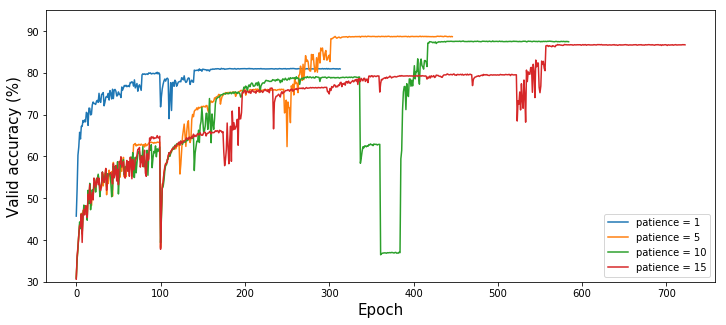
\includegraphics[width=0.7\linewidth]{figures/fig_patience.png}
    \vspace{-4mm}
	\caption{\small Effect of patience level on the validation accuracy trajectory during training. Each curve shows the validation accuracy on CIFAR-10 dataset.}
	\vspace{-4mm}
    \label{fig:patience}
\end{figure*}

\vspace{-2mm}
\section{Effect of training steps in the growth
\vspace{-2mm}
phase}\label{sec:supp_effect_of_patience}
Fig. \ref{fig:patience} compares the validation accuracies of the same ANT-CIFAR-C model trained on the CIFAR-10 dataset with varying levels of patience during early stopping in the growth phase. A higher patience level corresponds to more training epochs for optimising new modules in the growth phase. When the patience level is 1, the architecture growth terminates prematurely and plateaus at low accuracy at $80\%$. On the other hand, a patience level of 15 causes the model to overfit locally with  $87\%$. The patience level of 5 gives the best results with $91\%$ validation accuracy.

%A patience level of 1 leads the model to underfit with $80\%$ accuracy, while a patience level of 15 causes the model to overfit locally with  $87\%$ accuracy; in between these, the patience level of 5 gives the best results with a validation accuracy of $91\%$.}
%Figure. 1 shows that when too few steps of optimisation are performed e.g. patience level is 1, the architecture growth terminates prematurely and plateaus at low validation accuracy at 80\%, which is roughly 10\% lower than the best case with patience level of 5. On the other hand, if too many optimisation steps are taken e.g patience level 15, this causes the added component to overfit locally, and leads to nearly 4\% drop in accuracy. Tuning this hyperparameter of patience level is therefore integral to successful optimisations of ANTs.



\section{Expert specialisation}\label{sec:supp_expert_specialisation}
\vspace{-2mm}
We investigate if the learned routing strategy is meaningful by comparing the classification accuracy of our default path-wise inference against that of the predictions from the leaf node with the smallest reaching probability. Tab. \ref{tab:test_routers} shows that using the least likely ``expert" leads to a substantial drop in classification accuracy, down to close to that of random guess or even worse for large trees (ANT-MNIST-C and ANT-CIFAR10-C). This demonstrates that features in ANTs become specialised to the subsets of the partitioned input space at lower levels in the tree hierarchy. 

\begin{table}[h]
	\caption {Comparison of classification performance between the default single-path inference scheme and the prediction based on the least likely expert. \label{tab:test_routers}}
    \footnotesize
    \center
	\begin{tabular}{|l|c|c|}
		\hline
		\multicolumn{1}{|c}{\textbf{Module Spec.}} &  \multicolumn{1}{|c|}{\textbf{Error \%}} & \multicolumn{1}{c|}{\textbf{Error \%}}  \\
		&(Selected path) & (Least likely path)  \\
		\hline
		ANT-MNIST-A &0.69 & 86.18  \\
	    ANT-MNIST-B &0.73 & 81.98  \\
        ANT-MNIST-C &1.68 & 98.84  \\
		ANT-CIFAR10-A & 8.32 & 74.28  \\
        ANT-CIFAR10-B & 9.18 & 89.74  \\
        ANT-CIFAR10-C & 9.34 & 97.52  \\
		\hline
	\end{tabular}
\end{table}
\vspace{-4mm}
\section{Visualisation of discovered architectures}\label{sec:supp_architectures}
\vspace{-2mm}
Fig. \ref{fig:architectures} shows ANT architectures discovered on the MNIST (i-iii) and CIFAR-10 (iv-vi) datasets. We observe three notable trends. Firstly, a large proportion of the learned routers separate examples based on their classes (red histograms) with very high confidence (blue histograms). The ablation study in Sec.~5.~1 (Tab.~4 in the main text) shows that such hierarchical clustering benefits predictive performance, while the conditional computation enables more lightweight inference (Tab.~3 in the main text). Secondly, most architectures learn a few levels of features before resorting to primarily splits. However, over half of the architectures (ii-v) still learn further representations beyond the first split. Secondly, all architectures are unbalanced. This reflects the fact that some groups of samples may be easier to classify than others. This property is reflected by traditional DT algorithms, but not ``neural'' tree-structured models with pre-specified architectures \citep{laptev2014convolutional,frosst2017distilling,kontschieder2015deep,ioannou2016decision}. 
\begin{figure*}[ht]
	\center
	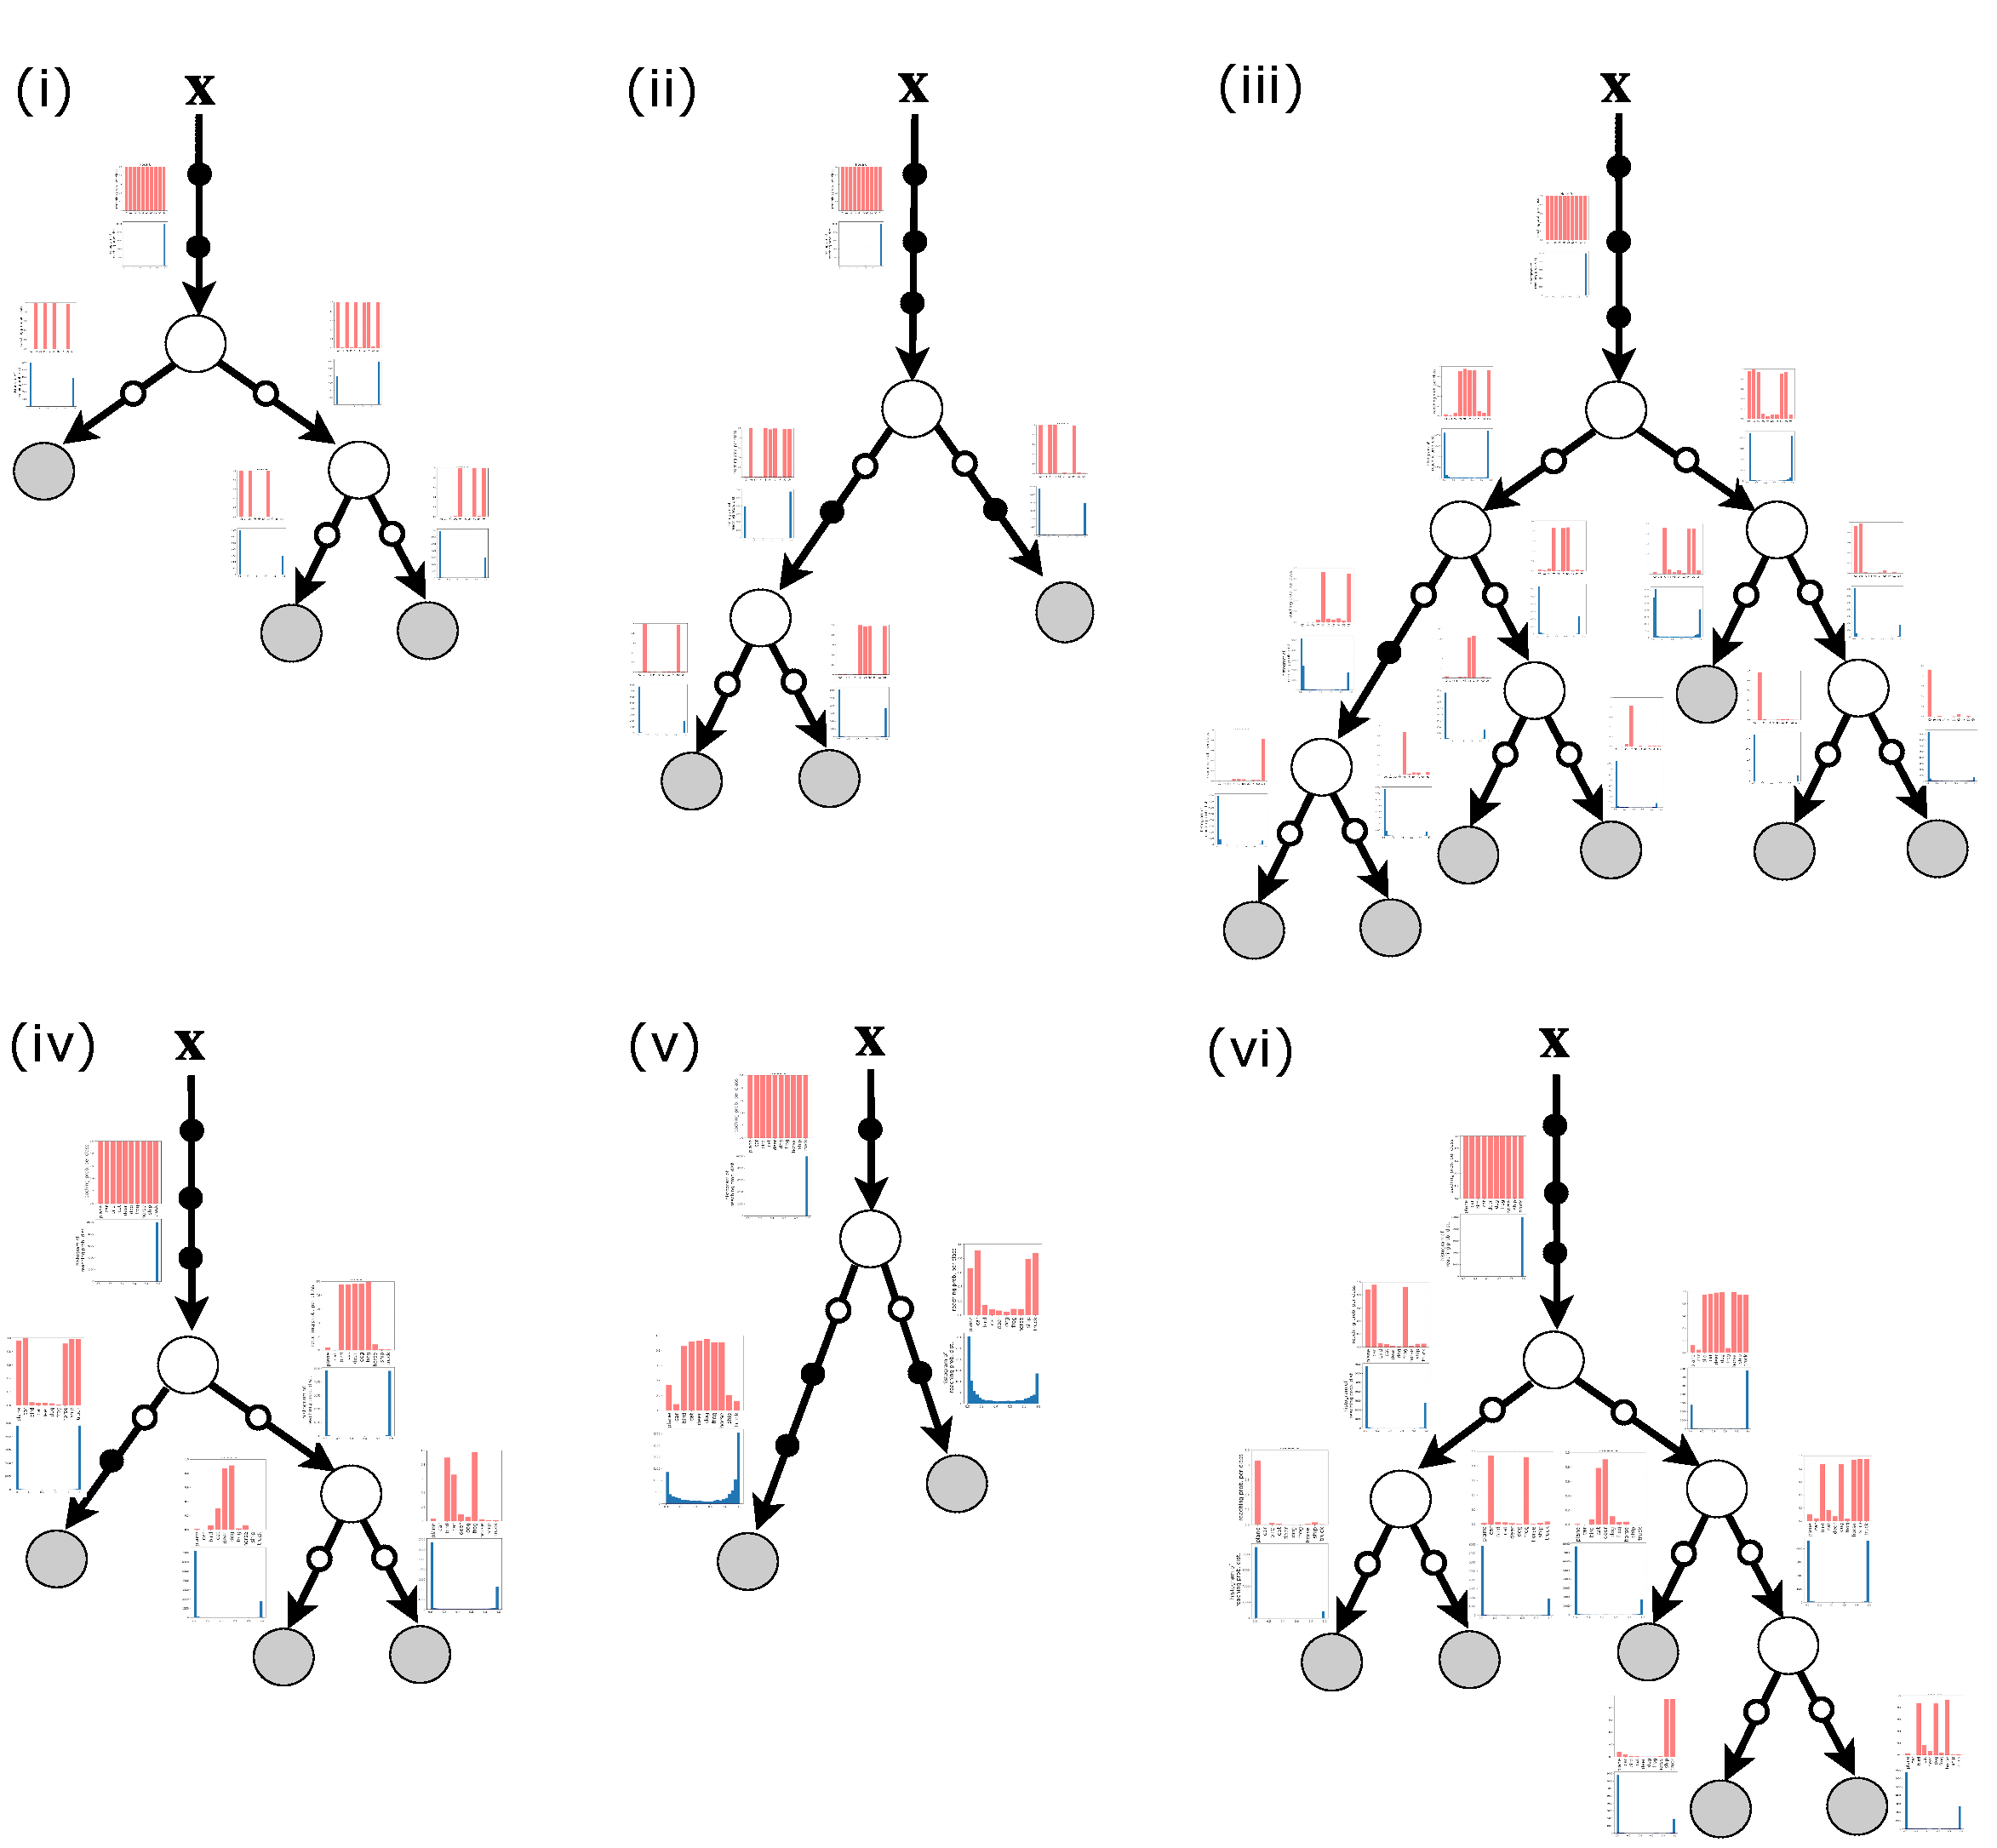
\includegraphics[width=0.8\linewidth]{figures/trees_all.pdf}
	\caption{\small Illustration of discovered ANT architectures. (i) ANT-MNIST-A, (ii) ANT-MNIST-B, (iii) ANT-MNIST-C, (iv) ANT-CIFAR10-A, (v) ANT-CIFAR10-B, (vi) ANT-CIFAR10-C. Histograms in red and blue show the class distributions and path probabilities at respective nodes. Small black circles on the edges represent transformers, circles in white at the internal nodes represent routers, and circles in gray are solvers. The small white circles on the edges denote specific cases where transformers are identity functions.}
	\label{fig:architectures}
\end{figure*}


% \section{Multivariate Regression}\label{sec:supp_regression}
% \vspace{-3mm}
% To demonstrate this, we also grow ANTs to perform (multivariate) regression on the SARCOS robot inverse dynamics dataset\footnote{\url{http://www.gaussianprocess.org/gpml/data/}}, which consists of 44,484 training and 4,449 testing examples, where the goal is to map from the 21-dimensional input space (7 joint positions, 7 joint velocities and 7 joint accelerations) to the corresponding 7 joint torques \citep{vijayakumar2000locally}. No dataset preprocessing or augmentation is used. We hold out 10\% of the training examples as a validation set. Baseline MLPs, routers and transformers are composed of single fully connected layers with 256 units with tanh nonlinearities, and the solver is a linear regressor. Other training details are the same as for classification (see Supp. Sec. \ref{sec:supp_train_details}). All non-NN-based methods were trained using scikit-learn \citep{pedregosa2011scikit}; only single-output GBT models were available so 7 separate GBTs were trained.

% The results are shown in Tab.~\ref{table:sarcos_results}. ANT-SARCOS outperforms all other methods in mean squared error with the full set of parameters, with GBTs performing slightly better using single-path inference. In comparison with results on MNIST and CIFAR-10, we note that the top 3 performing methods are all tree-based, with the third best method being an SDT (with MLP routers). This highlights the power of splitting the input space and conditional computation, both of which standard NNs are not capable of. Meanwhile, we still reap the benefits of representation learning, as shown by both ANT-SARCOS and the SDT (which is a specific form of ANT) requiring fewer parameters than the best-performing GBT configuration. Finally, we note that deeper NNs (5 vs. 3 hidden layers) can overfit on this small dataset, which makes the adaptive growth procedure of tree-based methods ideal for finding a model that exhibits good generalisation.

% \begin{table*}[ht]
% 	\caption{Comparison of performance of different models on SARCOS. The columns ``Error (Full)'' and ``Error (Path)'' indicate the mean squared error of predictions based on the full distribution and the single-path inference. The columns ``Params. (Full)'' and ``Params. (Path)'' respectively show the total number of parameters in the model and the average number of parameters utilised during single-path inference. ``Ensemble Size'' indicates the size of ensemble used to attain the reported accuracy. Results from \citet{zhao2017efficient} are included as a reference value from prior work, but are not directly comparable as they hold out 30\% of the training examples as a validation set.}
% 	\vspace{-3mm}
% 	\label{table:sarcos_results}
%     \center
%     \scriptsize
% 	\begin{tabular}{|c|l|cc|cc|c|}
% 		\hline
% 		& \multicolumn{1}{c|}{Method}
% 		& \multicolumn{1}{c}{\thead{\scriptsize Error \\ \scriptsize (Full)}}
% 		& \multicolumn{1}{c}{\thead{\scriptsize Error \\ \scriptsize (Path)}}
% 		& \multicolumn{1}{c}{\thead{\scriptsize Params. \\ \scriptsize (Full)}}
% 		& \multicolumn{1}{c|}{\thead{\scriptsize Params. \\ \scriptsize (Path)}}
% 		& \multicolumn{1}{c|}{\thead{\scriptsize Ensemble \\ \scriptsize Size}} \\	
% 		\hline
% 		\parbox[t]{2mm}{\multirow{11}{*}{\rotatebox[origin=c]{90}{SARCOS}}}
%         & Linear regression & 10.693 & N/A &\textbf{154}& N/A & 1 \\
%         & MLP with 2 hidden layers \citep{zhao2017efficient} & 5.111 & N/A & 31,804 & N/A & 1 \\
% 		& Decision tree & 3.708 & 3.708 & 319,591 & \textbf{25} & 1 \\
% 		& MLP with 1 hidden layer & 2.835 & N/A & 7,431 & N/A & 1 \\
%         & Gradient boosted trees & 2.661 & 2.661 & 391,324 & 2,083 & 7 $\times$ 30 \\
% 		& MLP with 5 hidden layers & 2.657 & N/A & 270,599 & N/A & 1 \\
% 		& Random forest & 2.426 & 2.426 & 40,436,840 & 4,791 & 200 \\
% 		& Random forest & 2.394 & 2.394 & 141,540,436 & 16,771 & 700 \\
% 		& MLP with 3 hidden layers & 2.129 & N/A & 139,015 & N/A & 1 \\
% 		&\cellcolor{gray!10}SDT (with MLP routers) &\cellcolor{gray!10} 2.118 &\cellcolor{gray!10} 2.246 &\cellcolor{gray!10} 28,045  &\cellcolor{gray!10} 10,167 &\cellcolor{gray!10} 1\\
% 		 & Gradient boosted trees & 1.444 & \textbf{1.444 }& 988,256 & 6,808 & 7 $\times$ 100 \\
% 		&\cellcolor{gray!10}ANT-SARCOS &\cellcolor{gray!10} \textbf{1.384} &\cellcolor{gray!10}  1.542 &\cellcolor{gray!10} 103,823  
% 		&\cellcolor{gray!10} 61,640 &\cellcolor{gray!10} 1\\
%       	\hline
% 	\end{tabular}
% \end{table*}

% \textbf{Ablation study:} we compare the regression error of our ANT in cases where the options for adding transformer or router modules are disabled (see Tab. \ref{tab:reg_ablationstudy}). In this experiment, patience levels are tuned separately for respective models. In the first case, the resulting models are equivalent to SDTs \citep{suarez1999globally} or HMEs \citep{jordan1994hierarchical} with locally grown architectures, while the second case is equivalent to standard NNs, grown adaptively layer by layer. We observe that either ablation consistently leads to higher regression errors across different module configurations. 
% \vspace{-3mm}
% \begin{table}[H]
% 	\caption{Ablation study to compare the effects of different components of ANTs on regression performance. ``NN'' refers to the case where the ANT is grown without routers while ``SDT/HME'' refers to the case where transformer modules on the edges are disabled. \label{tab:reg_ablationstudy}}
% 	\scriptsize
%     \center
% 	\begin{tabular}{|l|ccc|ccc|}
% 		\hline
% 		\multicolumn{1}{|c}{\textbf{Module Spec.}} &  \multicolumn{3}{|c|}{\textbf{Error (Full)}} & \multicolumn{3}{c|}{\textbf{ Error (Path)}} \\
% 			& ANT & NN & SDT/HME & ANT & NN & SDT/HME \\
% 			& (default) & (no routers) & (no transformers) & (default) & (no routers) & (no transformers) \\
% 		\hline
% 		ANT-SARCOS &1.384 & 2.511 & 2.118 &1.542 & 2.511 & 2.246 \\
% 		\hline
% 	\end{tabular}
% \end{table}
\vspace{-3mm}
\section{FLOPS}\label{sec:flops}
\vspace{-2mm}
Tab.\ref{tab:flops} reports the floating point operations per second (FLOPS) of ANT models for two inference schemes. The results for ResNet110 and DenseNet were retrieved from \cite{guan2017energy} and \cite{huang2018condensenet}, respectively. The FLOPs of all other models were computed using TorchStat toolbox available at \url{https://github.com/Swall0w/torchstat}. Using the single-inference reduces FLOPS in all ANT models to varying degrees.

\begin{table}[h]
% 	\caption {Comparison of classification performance between the default single-path inference scheme and the prediction based on the least likely expert. \label{tab:test_routers} between the }
    \caption{Comparison of FLOPs. \label{tab:flops}}
    \vspace{-5mm}
    \footnotesize
    \center
	\begin{tabular}{|c|l|c|c|}
		\hline
		&\multicolumn{1}{|c}{\textbf{Model}} &  \multicolumn{1}{|c|}{\textbf{FLOPS}} & \multicolumn{1}{c|}{\textbf{FLOPS}}  \\
		& &(multi-path) & (single-path)  \\
		\hline
		\parbox[t]{2mm}{\multirow{5}{*}{\rotatebox[origin=c]{90}{MNIST}}}
		&Linear Classifier & 8K & -   \\
		&LeNet-5 & 231 K & -  \\
		&ANT-MNIST-C & 99K & 83K  \\
	    &ANT-MNIST-B & 346K & 331K \\
        &ANT-MNIST-A & 382K & 380K  \\
        \hline
        
        \parbox[t]{2mm}{\multirow{7}{*}{\rotatebox[origin=c]{90}{CIFAR-10}}}&Net-in-Net & 222M &- \\
        &All-CNN & 245M & -\\
        &ResNet-110 & 256M&- \\
        &DenseNet-BC (k=24)& 9388M &- \\
		&ANT-CIFAR10-C & 66M & 61M  \\
        &ANT-CIFAR10-B & 163M & 149M  \\
        &ANT-CIFAR10-A & 254M & 243M  \\
		\hline
	\end{tabular}
\end{table}

\vspace{-5mm}
\section{Ensembling}\label{sec:supp_ensembling}
\vspace{-2mm}
As with traditional DTs \citep{breiman2001random} and NNs \citep{hansen1990neural}, ANTs can be ensembled to gain improved performance. In Tab.~\ref{tab:ensembling} we show the results of ensembling 8 ANTs (using the ``-A'' configurations for classification), each of which is trained with a randomly chosen split between training and validation sets. We compare against the single tree models, trained with the default split. In all cases both the multi-path and single-path inference performance is noticeably improved, and in MNIST we reach close to state-of-the-art performance (0.29\% versus 0.25\% \citep{sabour2017dynamic}) with significantly fewer parameters (851k versus 8.2M).
\vspace{-4mm}
\begin{table*}[ht]
	\caption{\small Comparison of prediction errors of a single ANT versus an ensemble of 8. \label{tab:ensembling}}
	\footnotesize
    \center
	\begin{tabular}{|l|cc|cc|cc|}
		\hline
		\multicolumn{1}{|c}{} &  \multicolumn{2}{|c|}{\textbf{MNIST} (Class Error \%)} &  \multicolumn{2}{|c|}{\textbf{CIFAR-10} (Class Error \%)} & \multicolumn{2}{c|}{\textbf{SARCOS} (MSE)}  \\
			& Multi-path & Single-path  & Multi-path & Single-path & Multi-path & Single-path   \\
		\hline
	    Single model & 0.64 & 0.69 & 8.31  & 8.32 & 1.384  & 1.542 \\	
        Ensemble & 0.29 & 0.30 & 7.76 & 7.79 & 1.226 & 1.372  \\
		\hline
	\end{tabular}
	\vspace{-4mm}
\end{table*}

\begin{table*}[ht]
	\caption{\small Parameter counts for a single ANT versus an ensemble of 8. \label{tab:ensembling_params}}
	\center
    \vspace{-1mm}
    \footnotesize
    \begin{tabular}{|l|cc|cc|cc|}
		\hline
		\multicolumn{1}{|c}{} &  \multicolumn{2}{|c|}{\textbf{MNIST} (No. Params.)} &  \multicolumn{2}{|c|}{\textbf{CIFAR-10} (No. Params.)} & \multicolumn{2}{c|}{\textbf{SARCOS}  (No. Params.)}  \\
			& Multi-path & Single-path  & Multi-path & Single-path & Multi-path & Single-path   \\
		\hline
	    Single model & 100,596 & 84,935 & 1.4M & 1.0M & 103,823 & 61,640 \\	
        Ensemble & 850,775 & 655,449 & 8.7M & 7.4M & 598,280 & 360,766  \\
		\hline
	\end{tabular}
	
	\vspace{-5mm}
\end{table*}



\clearpage
\clearpage

\bibliography{bibliography}
\bibliographystyle{icml2019}


\end{document}